L'évaluation des performances de l'EKF cinématique repose sur une comparaison
visuelle avec la vérité terrain Strava, acquise simultanément lors de trois
parcours distincts sur le campus de l'INSA Rouen. Chaque carte superpose
cinq couches : la vérité terrain Strava (noir), le GPS brut avant filtrage
(gris), le GPS nettoyé utilisé par le filtre (rouge), les points GPS rejetés
par le gate de Mahalanobis (orange), et la trajectoire estimée par l'EKF
(bleu).

\subsubsection{Terrain dégagé — grand parcours}

Sur un parcours de grande envergure en terrain dégagé
(Figure~\ref{fig:trajet_grand}), la trajectoire EKF (bleu) suit fidèlement
le GPS nettoyé (rouge) et reste à quelques mètres de la vérité terrain
Strava (noir). L'absence de points orange indique que le filtre de
Mahalanobis n'a rejeté aucune mesure GPS sur ce parcours : les conditions
extérieures dégagées produisent un signal GNSS de qualité, sans anomalie
détectable. La trajectoire EKF apparaît légèrement plus lisse que le GPS
nettoyé brut, ce qui confirme le rôle régularisateur du filtre.


\begin{figure}[H]
    \centering
    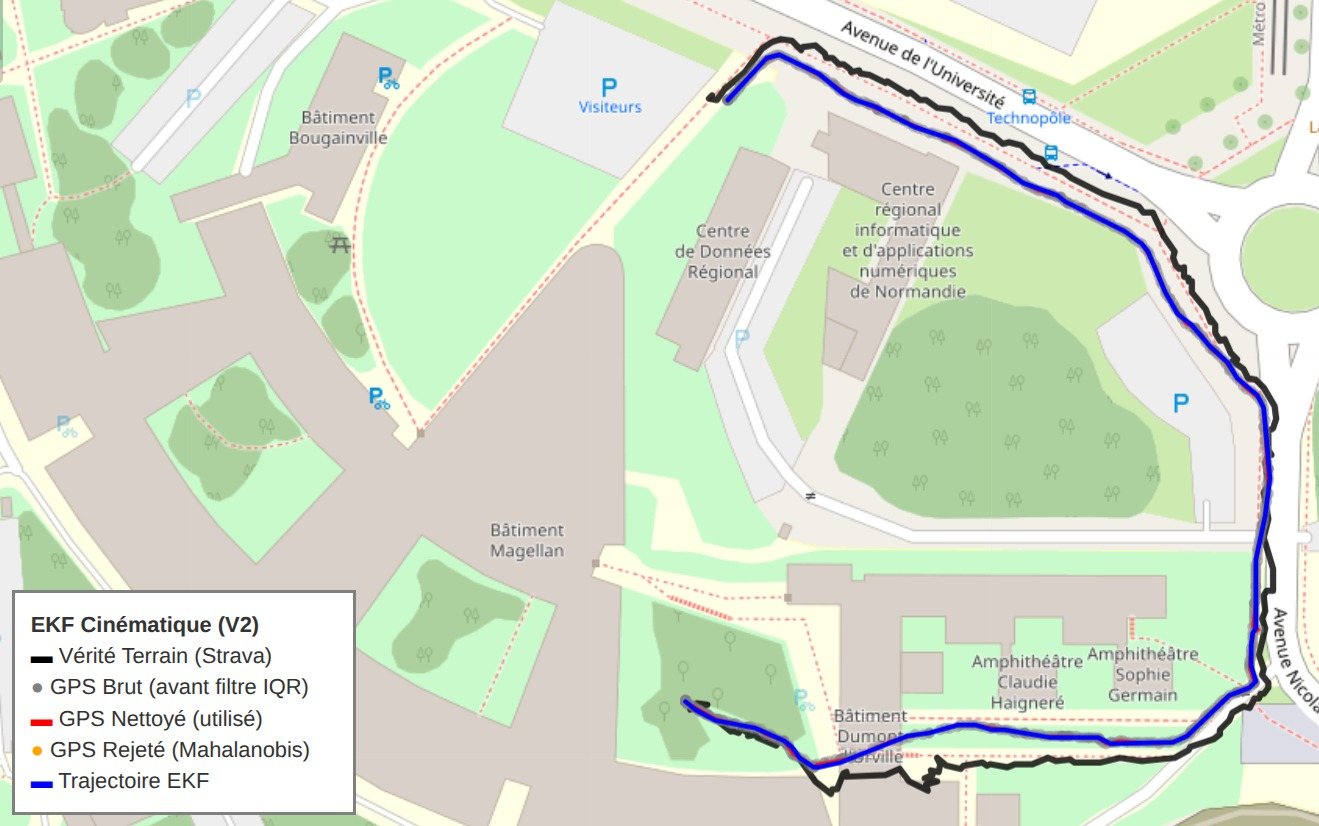
\includegraphics[width=0.65\textwidth]{images/trajet_plus_grand.jpeg}
    \caption{EKF cinématique sur grand parcours extérieur — campus INSA Rouen}
    \label{fig:trajet_grand}
\end{figure}



\subsubsection{Petit parcours — analyse des écarts}

Sur un trajet plus court (Figure~\ref{fig:trajet_petit}), un décalage
systématique apparaît entre notre estimation (rouge/bleu) et la vérité
terrain Strava (noir). Ce décalage, de l'ordre de quelques mètres, peut
s'expliquer par deux phénomènes distincts. D'une part, Strava utilise un
algorithme de \textit{map-matching} qui projette les positions GPS sur les
chemins connus de la carte, introduisant un biais artificiel par rapport
à la trajectoire réelle. D'autre part, l'imprécision résiduelle de notre
récepteur GNSS, modélisée par la matrice $R$, génère un décalage
incompressible même après filtrage. Ces deux sources d'erreur rendent
la comparaison absolue difficile, et justifient d'interpréter les résultats
de manière relative plutôt qu'absolue.


\begin{figure}[H]
    \centering
    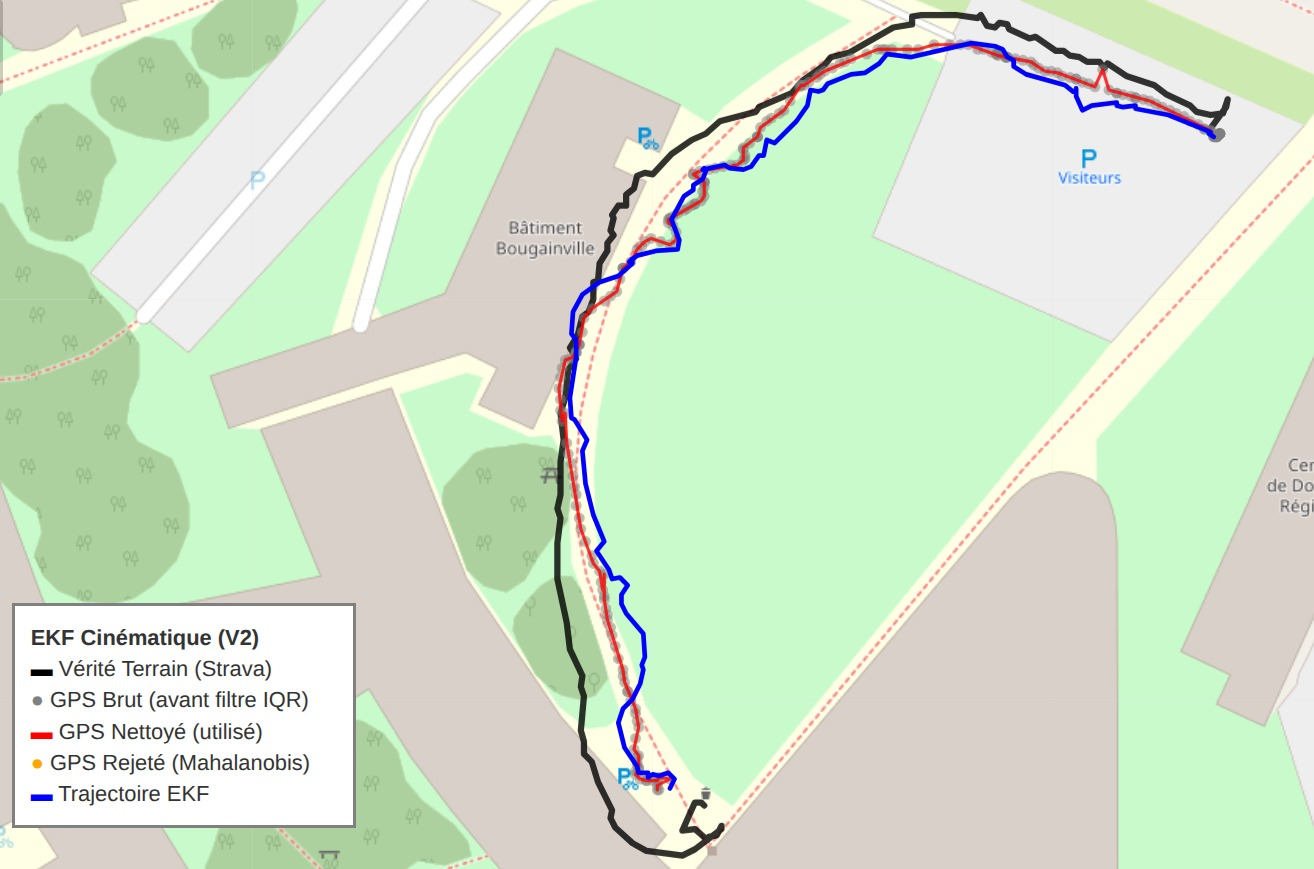
\includegraphics[width=0.65\textwidth]{images/trajet_petit.jpeg}
    \caption{EKF cinématique sur petit parcours — comparaison avec Strava}
    \label{fig:trajet_petit}
\end{figure}



\subsubsection{Passage en intérieur — robustesse du filtre}

Le troisième parcours (Figure~\ref{fig:trajet_ascenseur}) constitue le cas
le plus instructif. Lors d'un passage en intérieur (ascenseur et couloirs),
le signal GNSS subit de fortes perturbations de type \textit{multipath} :
les réflexions sur les murs produisent des positions aberrantes, visibles
sous forme d'un large nuage de points orange dans la partie inférieure de
la carte. Le gate de Mahalanobis a correctement identifié et rejeté
l'intégralité de ces mesures corrompues.

Durant cette phase de dégradation GPS, l'EKF a maintenu une trajectoire
continue et physiquement cohérente (bleu) en s'appuyant uniquement sur
le modèle cinématique. Ce comportement illustre concrètement l'apport de
la fusion multi-capteurs : là où un GPS seul produirait une trajectoire
erratique, le filtre de Kalman assure la continuité de l'estimation.

On notera que la vérité terrain Strava (noir) présente elle-même un
comportement erratique dans la même zone, confirmant que les perturbations
GNSS en intérieur affectent tous les récepteurs, y compris les smartphones
modernes.



\begin{figure}[H]
    \centering
    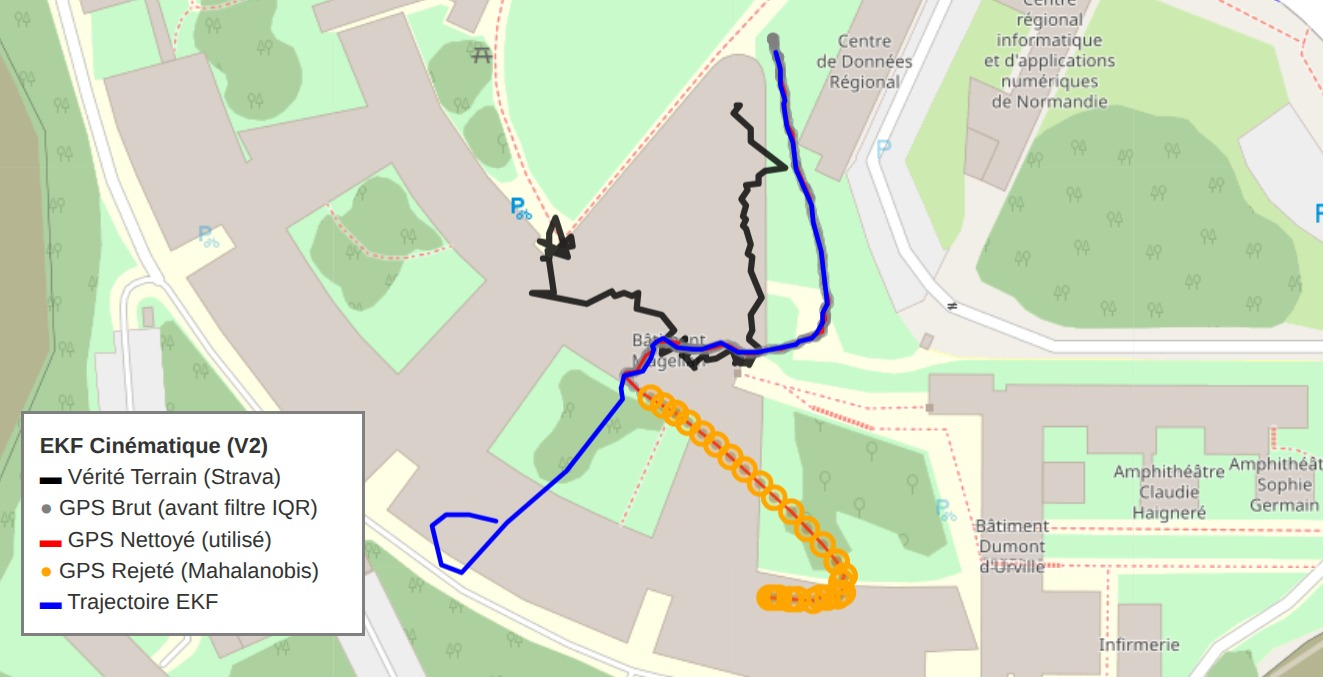
\includegraphics[width=0.65\textwidth]{images/trajet_avec_ascenceur.jpeg}
    \caption{Rejet Mahalanobis lors d'un passage en intérieur — EKF en navigation autonome}
    \label{fig:trajet_ascenseur}
\end{figure}



\subsubsection{Bilan}

Les trois acquisitions mettent en évidence les points suivants :

\begin{itemize}
    \item \textbf{En terrain dégagé}, l'EKF produit une trajectoire lisse
    et cohérente, très proche de la vérité terrain.
    \item \textbf{En conditions dégradées} (intérieur, multipath), le gate
    de Mahalanobis rejette efficacement les mesures corrompues et l'EKF
    maintient une estimation continue grâce au modèle cinématique.
    \item \textbf{Un décalage résiduel} de quelques mètres persiste entre
    notre estimation et Strava, attribuable en partie au map-matching de
    Strava et en partie à la précision intrinsèque du récepteur GNSS.
\end{itemize}